\documentclass{article}

\usepackage{fullpage}
\usepackage{url}
\usepackage{bbm}
\usepackage{graphicx}
\usepackage{amsmath}
\usepackage{physics}
\usepackage{mathtools}
\usepackage{bbold}
\usepackage{slashed}
\usepackage{pxfonts}
\usepackage{multicol}
\usepackage{mathptmx}
\usepackage{simplewick}
\usepackage{placeins}

\usepackage{lmodern}
\usepackage[T1]{fontenc}
\usepackage[fontsize=13.5pt]{fontsize}

\DeclareMathOperator{\erfi}{erfi}
\newcommand{\R}{\ensuremath{\mathbb{R}}}
\newcommand{\C}{\ensuremath{\mathbb{C}}}

\title{Quantum Field Theory I Excercise 4}
\author{Idan Stark}
\date{\today}

\begin{document}
\maketitle

\section{Pauli-Villars regularization}
\subsection{The $2 \rightarrow 2$ scattering amplitude in $\phi^4$ theory}
As we saw in class, for the $2 \rightarrow 2$ scattering in $\phi^4$ theory in $3 + 1$ dimensions:
\begin{equation}
    i\mathcal{M} = -i\lambda + (-i\lambda)^2\left[iV(s) + iV(t) + iV(u)\right] + O(\lambda^3)
\end{equation}
Where:
\begin{equation}
    V\left(p^2\right) = \frac{i}{2}\int \frac{d^4k}{(2\pi)^4}\frac{1}{k^2 - m^2 + i\epsilon}\frac{1}{(k + p)^2 - m^2 + i\epsilon}
\end{equation}
And $s, t, u$ are the Mandelstam variables. The integral in $V$ diverges, so let us calculate it using Pauli-Villars regularization:
\begin{equation}
\begin{gathered}
    \frac{1}{k^2 - m^2 + i\epsilon} \rightarrow \frac{1}{k^2 - m^2 + i\epsilon} - \frac{1}{k^2 - \Lambda^2 + i\epsilon}
    \\
    \frac{1}{(k + p)^2 - m^2 + i\epsilon} \rightarrow \frac{1}{(k + p)^2 - m^2 + i\epsilon} - \frac{1}{(k + p)^2 - \Lambda^2 + i\epsilon}
\end{gathered}
\end{equation}
Multiplying these two gives four terms, each one is a product of two such fractions:
\begin{equation}
\begin{gathered}
    V\left(p^2\right) = \frac{i}{2}\int \frac{d^4k}{(2\pi)^4} \times \\ \times \Bigg[
        \frac{1}{k^2 - m^2 + i\epsilon}\frac{1}{(k + p)^2 - m^2 + i\epsilon} -
        \frac{1}{k^2 - m^2 + i\epsilon}\frac{1}{(k + p)^2 - \Lambda^2 + i\epsilon} - \\ -
        \frac{1}{k^2 - \Lambda^2 + i\epsilon}\frac{1}{(k + p)^2 - m^2 + i\epsilon} +
        \frac{1}{k^2 - \Lambda^2 + i\epsilon}\frac{1}{(k + p)^2 - \Lambda^2 + i\epsilon}
    \Bigg]
\end{gathered}
\end{equation}
We can now combine the first and second term to get in the nominator:
\begin{equation}
\begin{gathered}
    \left[k^2 - m^2 + i\epsilon\right]\left[(k + p)^2 - \Lambda^2 + i\epsilon\right] - \left[k^2 - m^2 + i\epsilon\right]\left[(k + p)^2 - m^2 + i\epsilon\right] = \\ =\left(m^2 - \Lambda^2 + i\epsilon\right)\left(k^2 - m^2 + i\epsilon\right)
\end{gathered}
\end{equation}
And similarly with the third and fourth terms:
\begin{equation}
\begin{gathered}
    \left[k^2 - \Lambda^2 + i\epsilon\right]\left[(k + p)^2 - m^2 + i\epsilon\right] - \left[k^2 - \Lambda^2 + i\epsilon\right]\left[(k + p)^2 - \Lambda^2 + i\epsilon\right] = \\ = -\left(m^2 - \Lambda^2 + i\epsilon\right)\left(k^2 - \Lambda^2 + i\epsilon\right)
\end{gathered}
\end{equation}
The integral then becomes:
\begin{equation}
\begin{gathered}
    V\left(p^2\right) = \frac{i}{2}\int \frac{d^4k}{(2\pi)^4} \times \\ \times \Bigg[
        \frac{\left(m^2 - \Lambda^2 + i\epsilon\right)\left(k^2 - m^2 + i\epsilon\right)}{\left[k^2 - m^2 + i\epsilon\right]^2\left[(k + p)^2 - \Lambda^2 + i\epsilon\right]\left[(k + p)^2 - m^2 + i\epsilon\right]} - \\ -
        \frac{\left(m^2 - \Lambda^2 + i\epsilon\right)\left(k^2 - \Lambda^2 + i\epsilon\right)}{\left[k^2 - \Lambda^2 + i\epsilon\right]^2\left[(k + p)^2 - \Lambda^2 + i\epsilon\right]\left[(k + p)^2 - m^2 + i\epsilon\right]}
    \Bigg] = \\ =
    \frac{i}{2}\left(m^2 - \Lambda^2 + i\epsilon\right)\int \frac{d^4k}{(2\pi)^4}
    \frac{1}{\left[(k + p)^2 - \Lambda^2 + i\epsilon\right]\left[(k + p)^2 - m^2 + i\epsilon\right]}
    \times \\ \times \Bigg[
        \frac{1}{k^2 - m^2 + i\epsilon} -
        \frac{1}{k^2 - \Lambda^2 + i\epsilon}
    \Bigg]
\end{gathered}
\end{equation}
which clearly converges, since it goes as $k^{-6}d^4k \sim k^{-6}\cdot k^3 \sim k^{-3}$. This means that each pair of fractions cancel each other such that their sum converges. We can now write the integral as a sum of two integral, both of which converge:
\begin{equation}
\begin{gathered}
    V\left(p^2\right) = \\ =
    \frac{i}{2}\int \frac{d^4k}{(2\pi)^4}\Bigg[
        \frac{1}{k^2 - m^2 + i\epsilon}\frac{1}{(k + p)^2 - m^2 + i\epsilon} -
        \frac{1}{k^2 - m^2 + i\epsilon}\frac{1}{(k + p)^2 - \Lambda^2 + i\epsilon}
    \Bigg] + \\ +
    \frac{i}{2}\int \frac{d^4k}{(2\pi)^4}\Bigg[
        \frac{1}{k^2 - \Lambda^2 + i\epsilon}\frac{1}{(k + p)^2 - \Lambda^2 + i\epsilon} -
        \frac{1}{k^2 - \Lambda^2 + i\epsilon}\frac{1}{(k + p)^2 - m^2 + i\epsilon}
    \Bigg]
\end{gathered}
\end{equation}
From now on we will use the original integral, knowning that as the sum of the converging integrals, it also converges. Now, we can introduct a Feynman variable $x$:
\begin{equation}
    \frac{1}{AB} = \int_0^1 dx \frac{1}{\left[Ax + B(1 - x)\right]^2}
\end{equation}
All four terms can be written as:
\begin{equation}
\begin{gathered}
    \frac{1}{k^2 - m_1^2 + i\epsilon}\frac{1}{(k + p)^2 - m_2^2 + i\epsilon} = \\ = \int_0^1 \frac{dx}{\left[
        \left((k + p)^2 - m_2^2\right)x +
        \left(k^2 - m_1^2\right)(1 - x)
        + i\epsilon
    \right]^2} = \\ =
    \int_0^1 \frac{dx}{\left[
        k^2 + 2xp\cdot k + p^2 x - m_2^2 x - m_1^2(1 - x)
        + i\epsilon
    \right]^2} = \\ =
    \int_0^1 \frac{dx}{\left[
        k^2 + 2xp\cdot k + p^2 x + \left(m_1^2 - m_2^2\right) x - m_1^2
        + i\epsilon
    \right]^2}
\end{gathered}
\end{equation}
Defining $l = k + px$ gives:
\begin{equation}
\begin{gathered}
    \frac{1}{k^2 - m_1^2 + i\epsilon}\frac{1}{(k + p)^2 - m_2^2 + i\epsilon} = \\ =
    \int_0^1 \frac{dx}{\left[
        l^2 + x(1 - x) p^2  + \left(m_1^2 - m_2^2\right) x - m_1^2
        + i\epsilon
    \right]^2}
\end{gathered}
\end{equation}
This means that we can write the integral as (already exchanging the integration order, because we can):
\begin{equation}
\begin{gathered}
    V\left(p^2\right) = \frac{i}{2} \int_0^1 dx \int \frac{d^4l}{(2\pi)^4} \times \\ \times
    \Bigg[
        \frac{1}{\left[l^2 + x(1 - x) p^2 - m^2
        + i\epsilon\right]^2} -
        \frac{1}{\left[l^2 + x(1 - x) p^2 + \left(m^2 - \Lambda^2\right) x - m^2
        + i\epsilon\right]^2} + \\ +
        \frac{1}{\left[l^2 + x(1 - x) p^2 - \Lambda^2
        + i\epsilon\right]^2} -
        \frac{1}{\left[l^2 + x(1 - x) p^2 + \left(\Lambda^2 - m^2\right) x - \Lambda^2
        + i\epsilon\right]^2}
    \Bigg]
\end{gathered}
\end{equation}
Using $i\epsilon$ to move to Euclidean integral:
\begin{equation}
\begin{gathered}
    V\left(p^2\right) = -\frac{1}{2} \int_0^1 dx \int \frac{d^4l}{(2\pi)^4} \times \\ \times
    \Bigg[
        \frac{1}{\left[l^2 + x(1 - x) p^2 - m^2\right]^2} -
        \frac{1}{\left[l^2 + x(1 - x) p^2 + \left(m^2 - \Lambda^2\right) x - m^2\right]^2} + \\ +
        \frac{1}{\left[l^2 + x(1 - x) p^2 - \Lambda^2\right]^2} -
        \frac{1}{\left[l^2 + x(1 - x) p^2 + \left(\Lambda^2 - m^2\right) x - \Lambda^2\right]^2}
    \Bigg]
\end{gathered}
\end{equation}
Finally, defining $y = l^2, d^4l = 2\pi^2 l^3 dl = \pi^2 ydy$, gives:
\begin{equation}
\begin{gathered}
    V\left(p^2\right) = -\frac{\pi^2}{2(2\pi)^4} \int_0^1 dx \int \times \\ \times
    \Bigg[
        \frac{ydy}{\left[y + x(1 - x) p^2 - m^2\right]^2} -
        \frac{ydy}{\left[y + x(1 - x) p^2 + \left(m^2 - \Lambda^2\right) x - m^2\right]^2} + \\ +
        \frac{ydy}{\left[y + x(1 - x) p^2 - \Lambda^2\right]^2} -
        \frac{ydy}{\left[y + x(1 - x) p^2 + \left(\Lambda^2 - m^2\right) x - \Lambda^2\right]^2}
    \Bigg] = \\ =
    -\frac{\pi^2}{2(2\pi)^4} \int_0^1 dx \times \\ \times
    \Bigg[
        \frac{m^2 - x(1 - x) p^2}{m^2 - x(1 - x) p^2 - y} + \log(m^2 - x(1 - x) p^2 - y) - \\
        - \frac{m^2 - x(1 - x) p^2 - \left(m^2 - \Lambda^2\right) x}{m^2 - x(1 - x) p^2 - \left(m^2 - \Lambda^2\right) x - y} - \log(m^2 - x(1 - x) p^2 - \left(m^2 - \Lambda^2\right) x - y) + \\
        +
        \frac{\Lambda^2 - x(1 - x) p^2}{\Lambda^2 - x(1 - x) p^2 - y} + \log(\Lambda^2 - x(1 - x) p^2 - y) - \\
        -
        \frac{\Lambda^2 - x(1 - x) p^2 - \left(\Lambda^2 - m^2\right) x}{\Lambda^2 - x(1 - x) p^2 - \left(\Lambda^2 - m^2\right) x - y} - \log(\Lambda^2 - x(1 - x) p^2 - \left(\Lambda^2 - m^2\right) x - y) + \\
        + const
    \Bigg]_{y=0}^\infty =
\end{gathered}
\end{equation}
\begin{equation*}
\begin{gathered}
    = \frac{\pi^2}{2(2\pi)^4} \int_0^1 dx \times \\ \times
    \Bigg[
        \frac{m^2 - x(1 - x) p^2}{m^2 - x(1 - x) p^2} + \log(m^2 - x(1 - x) p^2) - \\
        - \frac{m^2 - x(1 - x) p^2 - \left(m^2 - \Lambda^2\right) x}{m^2 - x(1 - x) p^2 - \left(m^2 - \Lambda^2\right) x} - \log(m^2 - x(1 - x) p^2 - \left(m^2 - \Lambda^2\right) x) + \\
        +
        \frac{\Lambda^2 - x(1 - x) p^2}{\Lambda^2 - x(1 - x) p^2} + \log(\Lambda^2 - x(1 - x) p^2) - \\
        -
        \frac{\Lambda^2 - x(1 - x) p^2 - \left(\Lambda^2 - m^2\right) x}{\Lambda^2 - x(1 - x) p^2 - \left(\Lambda^2 - m^2\right) x} - \log(\Lambda^2 - x(1 - x) p^2 - \left(\Lambda^2 - m^2\right) x)
        + const
    \Bigg]
\end{gathered}
\end{equation*}
Where in the last step we used the fact that at $y \rightarrow \infty$, the fractions vanish and the logarithms cancel each other out. We can see that all the fractions cancel out to one, and thus become part of the cosntant. Taking $\Lambda \rightarrow \infty$, we can see that:
\begin{equation}
\begin{gathered}
    \log(\Lambda^2 - x(1 - x) p^2) - \log(\Lambda^2 - x(1 - x) p^2 - \left(\Lambda^2 - m^2\right) x) = \\ = \log(\frac{\Lambda^2 - x(1 - x) p^2}{\Lambda^2 - x(1 - x) p^2 - \left(\Lambda^2 - m^2\right) x}) \rightarrow \log(\frac{1}{1 - x}) = -\log(1 - x)
    \\
    \log(m^2 - x(1 - x) p^2) - \log(m^2 - x(1 - x) p^2 - \left(m^2 - \Lambda^2\right) x) = \\ = \log(\frac{m^2 - x(1 - x) p^2}{m^2 - x(1 - x) p^2 - \left(m^2 - \Lambda^2\right) x}) \rightarrow -\infty
\end{gathered}
\end{equation}
So:
\begin{equation}
\begin{gathered}
    V\left(p^2\right) \xrightarrow{\Lambda \rightarrow \infty}
    \frac{1}{32\pi^2} \int_0^1 dx
    \Bigg[
        \log(\frac{m^2 - x(1 - x) p^2}{m^2 - x(1 - x) p^2 - \left(m^2 - \Lambda^2\right) x}) - \log(1 - x) + const \Bigg]
\end{gathered}
\end{equation}
The second term is just a constant:
\begin{equation}
    \int_0^1 \log(1 - x) dx = \int_0^1 \log(x) dx = \left[x\log x - x\right]_0^1 = -1
\end{equation}
So, together with the integration constant, it doesn't depend on $p^2$:
\begin{equation}
\begin{gathered}
    V\left(p^2\right) \xrightarrow{\Lambda \rightarrow \infty}
    \frac{1}{32\pi^2} \int_0^1 dx
    \Bigg[
        \log(\frac{m^2 - x(1 - x) p^2}{m^2 - x(1 - x) p^2 - \left(m^2 - \Lambda^2\right) x})\Bigg] + const 
\end{gathered}
\end{equation}
Now, let us renormalize, as we saw in class, defining $\lambda_p$ as the scattering amplitude for $p_0^i = 0$ gives:
\begin{equation}
\begin{gathered}
    -\mathcal{M} = \lambda_p + \lambda_p^2 \left(V(s) - V(4m^2) + V(t) + V(u) - 2V(0)\right) = \\ =
    \lambda_p + \lambda_p^2 \frac{1}{32\pi^2} \int_0^1 dx \times \\ \times \Bigg[
        \log(\frac{m^2 - x(1 - x) s}{m^2 - x(1 - x) s - \left(m^2 - \Lambda^2\right) x})
        - \log(\frac{m^2 - x(1 - x) 4m^2}{m^2 - x(1 - x) 4m^2 - \left(m^2 - \Lambda^2\right) x}) + \\
        + \log(\frac{m^2 - x(1 - x) t}{m^2 - x(1 - x) t - \left(m^2 - \Lambda^2\right) x}) + \\
        + \log(\frac{m^2 - x(1 - x) u}{m^2 - x(1 - x) u - \left(m^2 - \Lambda^2\right) x})
        - 2\log(\frac{m^2}{m^2 - \left(m^2 - \Lambda^2\right) x})\Bigg] = \\ =
        \lambda_p + \lambda_p^2 \frac{1}{32\pi^2} \int_0^1 dx \times \\ \times \Bigg[
        \log(\frac{m^2 - x(1 - x) s}{m^2 - x(1 - x) 4m^2})
        + \log(\frac{m^2 - x(1 - x) t}{m^2}) + \log(\frac{m^2 - x(1 - x) u}{m^2})\Bigg]
\end{gathered}
\end{equation}
Where again we let the $\log(\Lambda)$ cancel each other out. We got the expected result!
\subsection{The connected contribution at order $\lambda$ to the 2-point
correlation function}
In the same theory, the two point correlation function $\langle T(\phi(x_1)\phi(x_2)) \rangle$ has a single diagram contributing in order $\lambda$, and that is the diagram we saw in class.
\begin{figure}[!htbp]
    \centering
    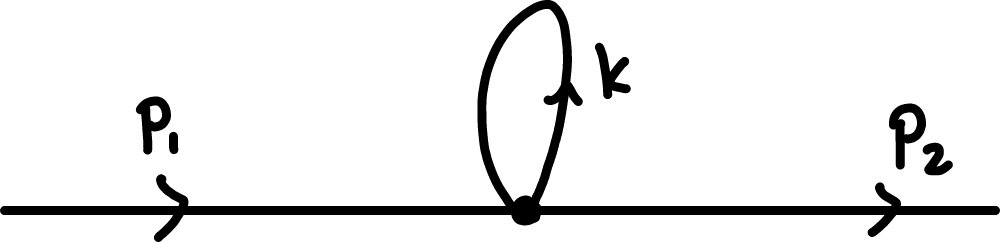
\includegraphics[width=0.5\textwidth]{figures/q1_2points.png}
    \caption{The diagram for the one vertex two points correlation function, identical to the one we saw in class.}
\end{figure}
It can be expressed using the momentum space Feynman rules to give (using a symmetry factor of 2):
\begin{equation}
\begin{gathered}
    \langle T(\phi(x_1)\phi(x_2)) \rangle = \frac{-i\lambda}{2}\int \frac{d^4k}{(2\pi)^4} \frac{d^4p_1}{(2\pi)^4} \frac{d^4p_2}{(2\pi)^4} \times \\ \times
    \frac{i(2\pi)^4\delta(p_1 + k - k + p_2)}{k^2 - m^2 + i\epsilon}\frac{ie^{-ip_1x_1}}{p_1^2 - m^2 + i\epsilon}\frac{ie^{-ip_2x_2}}{p_2^2 - m^2 + i\epsilon} = \\ =
    \frac{-i\lambda}{2}\int \frac{d^4k}{(2\pi)^4} \frac{d^4p}{(2\pi)^4}
    \frac{i}{k^2 - m^2 + i\epsilon}\frac{ie^{-ipx_1}}{p^2 - m^2 + i\epsilon}\frac{ie^{ipx_2}}{p^2 - m^2 + i\epsilon} = \\ =
    \frac{-i\lambda}{2}\int  \frac{d^4p}{(2\pi)^4} \left(\frac{i}{p^2 - m^2 + i\epsilon}\right)^2 e^{-ip\left(x_1 - x_2\right)}
    \int \frac{d^4k}{(2\pi)^4} \frac{i}{k^2 - m^2 + i\epsilon}
\end{gathered}
\end{equation}
This expression obviously diverges from the integral over $d^4k\cdot k^{-2} \sim k^3\cdot k^{-2} = k^{1}$. As we saw in the previous section, the Pauli-Villars regularization allows us to write such fractions as a sum that reduces their power by one (from multiplying the fractions and seeing that the $k^2$ factor in the nominator cancel out). This means that for this case we will get $k^{-1}$ which will diverge, so the Pauli-Villars regularization will not work in this case.
\newline
However, dimensional regularization will work here since this integral in dimension $d$ goes like $d^dk\cdot k^{-2} \sim k^{d - 3}$. So, it will converge for $d < 2$, there we can get a $\Gamma$ function and extend it back to $d = 4 - \epsilon$.

\newpage
\section{Scalar field theory in arbitrary dimensions}
Let us consider the d space-time field theory with Lagrangian density
\begin{equation}
    \mathcal{L} = \frac{1}{2}\partial^\mu\phi\partial_\mu\phi - \frac{1}{2}m^2\phi^2 - V(\phi)
\end{equation}
Where $V(\phi)$ is some potential that goes as a power law $\propto \phi^n$. The superficial DOF is:
\begin{equation}
    D = d + \left(n\left(\frac{d - 2}{2}\right) - d\right)V - \frac{d - 2}{2}N
\end{equation}
In general we require that for any number of external legs $N$, the more vertices we add the more exact the theory will be. This can be expressed in the requirement that the first term will not be positive:
\begin{equation}
    \boxed{n\left(\frac{d - 2}{2}\right) - d \le 0}
\end{equation}
Where we required 
\subsection{In $d = 3$}
The above relation gives
\begin{equation}
    n \le 6
\end{equation}
And so the allowed terms are:
\begin{equation}
    V(\phi) = \frac{\lambda_3}{3!}\phi^3 + \frac{\lambda_4}{4!}\phi^4 + \frac{\lambda_5}{5!}\phi^5 + \frac{\lambda_6}{6!}\phi^6
\end{equation}
\subsection{In $d = 2$}
From the above relation we can see that for $d = 2$ the equation is solved for every $n$, and so every possible theory is allowed.

\newpage
\section{One-loop renormalization of $\phi^3$ theory in four dimensions }
Let us consider the Lagrangian for a massive real scalar field with cubic self-interaction, in $d = 4$:
\begin{equation}
    \mathcal{L} = \frac{1}{2}\partial^\mu\phi\partial_\mu\phi - \frac{1}{2}m^2\phi^2 - \frac{g}{3!}\phi^3
\end{equation}
\subsection{The superficial degree of freedom}
using the equation, with $d = 4$ and $n = 3$, we get:
\begin{equation}
    D = 4 + \left(3 \cdot \frac{4 - 2}{2} - 4\right)V - \frac{4 - 2}{2}N
\end{equation}
\begin{equation}
    D = 4 - V - N
\end{equation}
Since the addition of both external legs and vertices make the superficial degree of freedom smaller, there is only a finite number of diagrams that are divergent, those with $N + V < 4$. This means the theory is considered super-renormalizable.
\subsection{Diverging daigrams}
So, we can consider the diagrams that diverge. Going one by one by number of external legs:
\begin{itemize}
    \item For $N = 1$, we considered all such diagrams to vanish.
    \item For $N = 2$, we require $V = 1, 2$, meaning that for the two-point correlation function we allow up to second order in perturbation theory. Since this is an odd power theory, we require the number of contracting fields to be even, and thus an even number of external legs requires an even number of vertices. This means that the only option for $N = 2$ is $V = 2$, which is manifest in the single loop diagram.
    \item For $N = 3$ we require $V = 1$, which is simply the single vertex with three external legs. This diagram doesn't diverge in reality since it has no internal propegators, there is no integral to diverge.
\end{itemize}

\newpage
\section{The $\phi^3$ theory in six dimensions}
Let us consdier, in the $\phi^3$ theory in $d = 6$:
\begin{equation}
    \mathcal{L} = \frac{1}{2}\partial^\mu\phi\partial_\mu\phi - \frac{1}{2}m^2\phi^2 - \frac{g}{3!}\phi^3
\end{equation}
the three point correlation function in momentum space:
\begin{equation}
    \langle \tilde{\phi}(p_1) \tilde{\phi}(p_2) \tilde{\phi}(p_3) \rangle
\end{equation}
\subsection{Renormalizability}
As we saw, the superficial degree of freedom for $d = 6, n = 3$ is:
\begin{equation}
    D = 6 + \left(3\left(\frac{6 - 2}{2}\right) - 6\right)V - \frac{6 - 2}{2}N =
    6 - 2N
\end{equation}
So, we notice that no matter how many vertices we add to the diagram, for $N \le 3$ it will diverge logarithmically while for $N > 3$ it will converge. This means the only diverging correlation functions are the two point correlation function and the three points correlation function, while every N point correlation function with $N > 3$ will always converge, making this theory renormalizable.
\subsection{First order correction}
Since this theory has an odd power $n = 3$, we can conclude that for odd number of legs $N = 3$, only odd number of vertices are allowed. In particular, in order $g$ with a single vertex we get the first contribution, and the first correction comes from the loop diagram with three legs at order $g^3$.
\begin{figure}[!htbp]
    \centering
    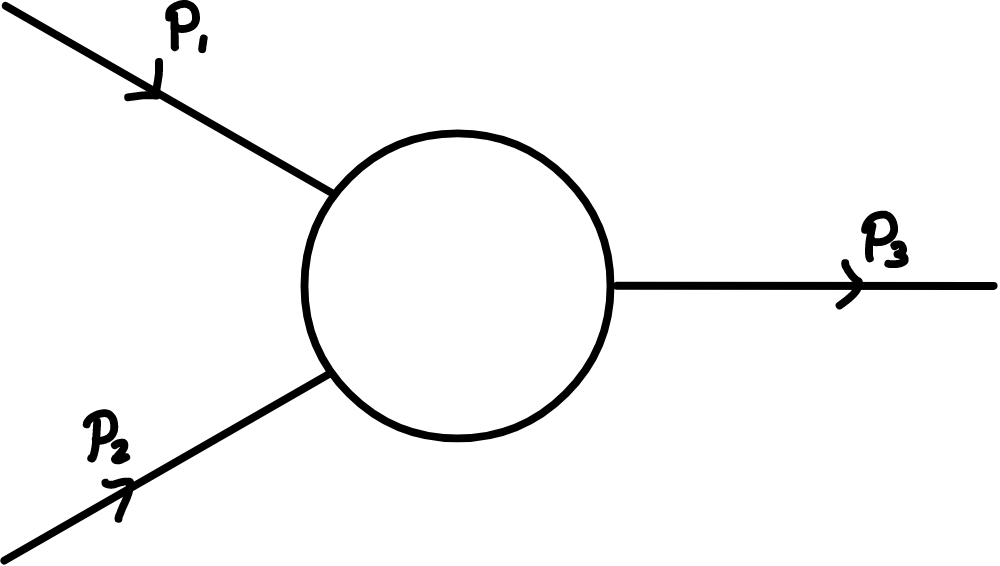
\includegraphics[width=0.5\textwidth]{figures/q4_3points.png}
    \caption{The three points loop diagram, which is the single third order diagram contributing to the three points correlation function.}
\end{figure}
\subsection{Copmuting the first order correction}
Using the momentum space Feynman rules, we get the expression:
\begin{equation}
\begin{gathered}
    \langle \tilde{\phi}(p_1) \tilde{\phi}(p_2) \tilde{\phi}(p_3) \rangle =
    (-ig)^3 \int \frac{d^6k_1}{(2\pi)^6} \frac{d^6k_2}{(2\pi)^6} \frac{d^6k_3}{(2\pi)^6} \times \\ \times
    (2\pi)^6\delta(p_1 + k_1 - k_2)(2\pi)^6\delta(p_2 + k_2 - k_3)(2\pi)^6\delta(p_3 + k_3 - k_1) \times \\ \times
    \frac{i}{k_1^2 - m^2 + i\epsilon}\frac{i}{k_2^2 - m^2 + i\epsilon}\frac{i}{k_3^2 - m^2 + i\epsilon}
\end{gathered}
\end{equation}
From the $\delta$ functions we get:
\begin{equation}
\begin{gathered}
    \delta(p_1 + k_1 - k_2) \rightarrow k_2 = p_1 + k_1 \\
    \delta(p_3 + k_3 - k_1) \rightarrow k_3 = k_1 - p_3 \\
    \delta(p_2 + k_2 - k_3) \rightarrow p_1 + p_2 + p_3 = k_2 - k_1 - k_3 + k_1 + k_3 - k_2 = 0
\end{gathered}
\end{equation}
So, renaming $k_1 = k$, we can use them to integrate over $k_2 = p_1 + k$ and $k_3 = k - p_3$, leaving us with a single $d^6k$ integral and a delta function for the conservation of the total momentum $\delta(p_1 + p_2 + p_3)$:
\begin{equation}
\begin{gathered}
    \langle \tilde{\phi}(p_1) \tilde{\phi}(p_2) \tilde{\phi}(p_3) \rangle =
    (-ig)^3 (2\pi)^6\delta \left(p_1 + p_2 + p_3\right) \times \\ \times
    \int \frac{d^6k}{(2\pi)^6}
    \frac{i}{k^2 - m^2 + i\epsilon}\frac{i}{(k + p_1)^2 - m^2 + i\epsilon}\frac{i}{(k - p_3)^2 - m^2 + i\epsilon}
\end{gathered}
\end{equation}
This integral acts like $d^6k \left(k^{-2}\right)^3 \sim k^5k^{-6}dk = k^{-1}dk$ which converges logarithmically, as expected. So, to regularize it, we will use dimensioanl regularization. Let us calculate then:
\begin{equation}
    V_d(p, q) = \int \frac{d^dk}{(2\pi)^d}
    \frac{i}{k^2 - m^2 + i\epsilon}\frac{i}{(k + p)^2 - m^2 + i\epsilon}\frac{i}{(k + q)^2 - m^2 + i\epsilon}
\end{equation}
Using Feynman's trick:
\begin{equation}
    \frac{1}{ABC} = 2\int_0^1 dx \int_0^{1-x} dy \frac{1}{\left[Ax + By + C(1 - x - y)\right]^3}
\end{equation}
This gives (after changing the order of integration):
\begin{equation}
\begin{gathered}
    V_d(p, q) = -2i \int_0^1 dx \int_0^{1-x} dy\int \frac{d^dk}{(2\pi)^d} \times \\ \times
    \frac{1}{\left(k^2 - m^2\right)(1 - x - y) + \left((k + p)^2 - m^2\right)y + \left((k + q)^2 - m^2\right)x + i\epsilon} = \\ =
    -2i \int_0^1 dx \int_0^{1-x} dy\int \frac{d^dk}{(2\pi)^d}
    \frac{1}{k^2 + 2(py + qx)k + p^2y + q^2x - m^2 + i\epsilon}
\end{gathered}
\end{equation}
Now, defining as in class $l = k + py + qx$ will give:
\begin{equation}
    V_d(p, q) =
    -2i \int_0^1 dx \int_0^{1-x} dy\int \frac{d^dl}{(2\pi)^d}
    \frac{1}{l^2 + (py + qx)^2 + p^2y + q^2x - m^2 + i\epsilon}
\end{equation}
Moving to Euclidean coordinates:
\begin{equation}
    V_d(p, q) =
    -2 \int_0^1 dx \int_0^{1-x} dy\int \frac{d^dl}{(2\pi)^d}
    \frac{1}{l^2 - (py + qx)^2 + p^2y + q^2x + m^2}
\end{equation}
And using the known integral:
\begin{equation}
    V_d(p, q) =
    -2 \int_0^1 dx \int_0^{1-x} dy
    \frac{\Gamma\left(3 - \frac{d}{2}\right)}{2\left(4\pi\right)^{d/2}}
    \left[m^2 - (py + qx)^2 - p^2y - q^2x\right]^{d/2 - 3}
\end{equation}
And taking $d \rightarrow 6 - \epsilon$ gives:
\begin{equation}
\begin{gathered}
    V(p, q) =
    -\frac{\Gamma\left(-\frac{\epsilon}{2}\right)}{\left(4\pi\right)^{3 - \epsilon/2}}
     \int_0^1 dx \int_0^{1-x} dy
    \left[m^2 - (py + qx)^2 - p^2y - q^2x\right]^{-\epsilon/2} = \\ =
    -\frac{\frac{2}{\epsilon} - \gamma}{\left(4\pi\right)^{3}}
     \int_0^1 dx \int_0^{1-x} dy
    \left(1 - \epsilon\ln(2\pi \left(m^2 - (py + qx)^2 - p^2y - q^2x\right))\right) = \\ =
    -\frac{1}{\left(4\pi\right)^{3}}
     \int_0^1 dx \int_0^{1-x} dy
    \left(\frac{2}{\epsilon} - \gamma + 2\ln(\pi \left(m^2 - (py + qx)^2 - p^2y - q^2x\right))\right)
\end{gathered}
\end{equation}
Som we can finally write the third order correction:
\begin{equation}
\begin{gathered}
    \langle \tilde{\phi}(p_1) \tilde{\phi}(p_2) \tilde{\phi}(p_3) \rangle_3 =
    -ig^3 \lim_{\epsilon \rightarrow 0}
    \frac{1}{64\pi^3}
    \times \\ \times
    \int_0^1 dx \int_0^{1-x} dy
    \left[\frac{2}{\epsilon} - \gamma + 2\ln(\pi \left(m^2 - (py + qx)^2 - p^2y - q^2x\right))\right]
    \times \\ \times
    (2\pi)^6\delta \left(p_1 + p_2 + p_3\right)
\end{gathered}
\end{equation}
And the full correlation funciton up to third order:
\begin{equation}
\begin{gathered}
    \langle \tilde{\phi}(p_1) \tilde{\phi}(p_2) \tilde{\phi}(p_3) \rangle =
    -ig - ig^3 \lim_{\epsilon \rightarrow 0}
    \frac{1}{64\pi^3}
    \times \\ \times
    \int_0^1 dx \int_0^{1-x} dy
    \left[\frac{2}{\epsilon} - \gamma + 2\ln(\pi \left(m^2 - (py + qx)^2 - p^2y - q^2x\right))\right]
    \times \\ \times
    (2\pi)^6\delta \left(p_1 + p_2 + p_3\right)
\end{gathered}
\end{equation}
\subsection{Defining a physical constant $g_p$}
We can define the constant as the correlation function with $p_1 = p_3 = 0$. This will give:
\begin{equation}
    g_p = g + g^3 \frac{1}{64\pi^3} \int_0^1 dx \int_0^{1-x} dy
    \left[\frac{2}{\epsilon} - \gamma + 2\ln(\pi m^2)\right]
\end{equation}
We can now invrese the relation:
\begin{equation}
    g = g_p - g_p^3\frac{1}{64\pi^3} \int_0^1 dx \int_0^{1-x} dy
    \left[\frac{2}{\epsilon} - \gamma + 2\ln(\pi m^2)\right]
\end{equation}
And plugging this back into the correcltion function gives:
\begin{equation}
\begin{gathered}
    -i\left(g_p - g_p^3\frac{1}{64\pi^3} \int_0^1 dx \int_0^{1-x} dy
    \left[\frac{2}{\epsilon} - \gamma + 2\ln(\pi m^2)\right]\right)
    - ig_p^3 \lim_{\epsilon \rightarrow 0}
    \frac{1}{64\pi^3}
    \times \\ \times
    \int_0^1 dx \int_0^{1-x} dy
    \left[\frac{2}{\epsilon} - \gamma + 2\ln(\pi \left(m^2 - (py + qx)^2 - p^2y - q^2x\right))\right]
    \times \\ \times
    (2\pi)^6\delta \left(p_1 + p_2 + p_3\right) = \\ =
    -ig_p - ig_p^3 \frac{1}{32\pi^3}
    \int_0^1 dx \int_0^{1-x} dy
    \ln(\frac{m^2 - (py + qx)^2 - p^2y - q^2x}{m^2})
\end{gathered}
\end{equation}
\end{document}